\section{Field of View Vignette}\label{sec:field-of-view-vignette}

One of the most common methods to reduce cybersickness risks and symptoms is decreasing the Field of
View as examined in section~\ref{subsec:field-of-view-limitation}.
To alleviate cybersickness during movements with high detail, and movements in the peripheral areas of vision, a
vignette is implemented to limit the Field of View, focusing the users attention and preventing the influence of
activity in the peripheral vision from adding to cybersickness symptoms.
The Vignette is primarily planned for movements close to an object's surface, where peripheral visual flow is
significantly higher compared to movements in interplanetary space.
Additionally, reducing the FoV may help users during the adaption phase, by directing their view to the center of the
HMD's lenses where the image is focused.
While a point of interest is within a users field of view, they tend to shift their gaze without moving their head.
This can lead to users trying to focus on objects that are not at the center of their view, and thereby not in the
center of the HMD lenses.
In this case the user is trying to focus on part of the virtual environment, that cannot be focused on based on
hardware limitations.
A FoV vignette can help the adaptation process by limiting the FoV and nudging the user towards using head movements
instead of eye movements to look at different points of interest and keep their gaze centered at the middle of the
HMD's lenses.
However, these adaptation aids require a narrow FoV and may be perceived as limiting or annoying to other users.
According to the best practices by McCauley and Sharkey~\cite{McCauley1992}, and similar to the Floor Grid, the
vignette is designed to be modular and adaptable to each individual user.
Additionally, several options of vignetting are implemented, as suggested by Lim et al.~\cite{Lim2020}, to allow the
user options for both dynamic and fixed limitation of FoV\@.


\subsection{FoV Vignette Implementation}\label{subsec:fov-vignette-implementation}

\begin{figure}[h]
    \centering
    \includegraphics[width=\textwidth]{content/4_2_fovVignette/img/Vignette_Screenshot}
    \caption{Screenshot of CosmoScout VR with (right) and without (left) the FoV Vignette.}
    \label{fig:fov-vignette-screenshot}
\end{figure}
The FoV Vignette is also implemented in the VR Accessibility Plugin for CosmoScout VR, together with the Floor Grid.
The vignette is realized as a post-processing shader, drawing a 2D effect over the rendered scene based on an
inner and outer radius, which are both adjustable in the settings.
The inner radius determines the maximum distance from the center of the viewport, where a clear field of view is
guaranteed.
The outer radius determines the minimum distance from the center, above which the screen is fully opaque with a custom
color that is also adjustable in the settings.
The area between the inner and outer radius is bridged by a gradient, blending between fully transparent, showing the
rendered scene, and the fully opaque custom color at the outer radius.
Since the vignette is designed to block peripheral visual flow inducing vection and distracting the user during
movement, the vignette is only drawn during movement, and disabled when standing still or during sporadic, short
movements.
This allows reducing the risk of cybersickness symptoms during critical phases, while still maintaining the feeling
of presence as much as possible.
As mentioned above, two different methods of vignetting are implemented to offer more customization to the user.
One method is drawing the vignette dynamically based on the observer's velocity in relation to the Observer's
position and distance to other bodies, as interplanetary movements allow for, and use significantly higher
velocities than movements close to a bodies surface.
For more customisation, an adjustable upper and lower velocity threshold for this normalized velocity is given to
allow more sensitive users an earlier and more noticeable vignetting, and more robust users the freedom to reduce its
effects.
The lower velocity threshold is the velocity at which the vignette will start limiting the FoV by decreasing its
radius, and the upper velocity threshold is the velocity where the vignette is at a determined minimum radius.
An adjustable threshold for the minimum velocity is used, since slow movements tend to only produce low risks of
cybersickness symptoms and limiting the FoV is usually not necessary.
Providing an upper velocity threshold serves solves two problems, it allows sensitive users to benefit of a
drastically reduced FoV as early as they feel comfortable, and additionally preventing the vignette from jittering
at maximum velocity where the velocity tends to fluctuate slightly, propagating to the radii of the dynamic vignette.
The FoV vignette is drawn in the same way for both options as shown in the fragment shader for the dynamic radius:
\begin{minted}{c}
    void main()
    {
        if (uNormVelocity <= 0 && !uDebug ) { discard; }

        vec2 texSize = textureSize(uTexture, 0);
        float ratio = texSize.y / texSize.x;

        float dist = sqrt(vPosition.x * vPosition.x + ratio * ratio * vPosition.y * vPosition.y);

        if (dist < uInnerRadius ) { discard; }
        float r = ((dist - uInnerRadius) / (uOuterRadius - uInnerRadius));
        oColor = mix(texture(uTexture, vTexCoords), uCustomColor, r);
        if (dist > uOuterRadius) {
          oColor.rgb = uCustomColor.rgb;
        }
    }
\end{minted}
The debug flag (\textit{uDebug}) exists to allow for easy adjustments of the vignette's variables, and if enabled
draws the vignette with its minimum radius.
First the distance (\textit{dist}) of the current fragment to the center of the viewport is calculated and adjusted
for the viewport's aspect ratio (\textit{ratio}).
Based on this distance and the inner and outer radius (\textit{uInnerRadius} and \textit{uOuterRadius}) the blending
factor (\textit{r}) is calculated, and the rendered scene (\textit{uTexture}) is blended with the custom color to
create the gradient between the inner and outer radius.
If the fragment is inside the inner radius, the post processing is discarded,a nd if the fragment is outside the
outer radius it is set to the color of the vignette (\textit{uCustomColor}).
The dynamic vignette's radius is controlled through the inner and outer radius that is passed to the fragment shader,
and is updated during the update frames of the simulation.
In the update the velocity is normalized to the upper and lower velocity threshold, and a new radius is calculated
partly based on the previous radius to dampen the propagation of harsh changes in velocity and smoothen the changes
in radii.
Currently, new radii propagate with a 1\% influence over each frame:
\begin{equation}
    \label{eq:radii-influence}
    r_{new} = ( 0.99 \times r_{last} ) + ( 0.01 \times r_{target} )
\end{equation}

As suggested by Lim et al.~\cite{Lim2020}, an option for a fixed vignette is also implemented.
The fixed vignette also uses the lower velocity threshold to determine when it should be drawn.
Additionally, an adjustable deadzone is implemented, allowing for a grace period where the vignette is not displayed
when passing the threshold to avoid flickering on short, quick movements, or velocities close to the threshold, that
pass the threshold when fluctuating slightly.
After passing the velocity threshold for at least the deadzone time or longer, a fade animation is used to ease the
vignette in or out over an adjustable duration, to make the transition to the limited field of view more comfortable and
less noticeable.
Through the use of an animation to gradually increase the opacity of the Vignette, a closing movement similar to the
dynamic vignette along the gradient is suggested.
However, the vignette is independent of the velocity, and is drawn with its specified minimum radius as soon as the
lower velocity threshold is passed.
As with the Floor Grid, almost all settings specifying the FoV vignette are adjustable either in the settings
file, or in the options menu at runtime, to allow users to customise the vignette according to their hardware setup
and preferences.

Finally, an experimental option is implemented, to only limit the FoV vertically and asymmetrically.
\begin{figure}[h]
    \centering
    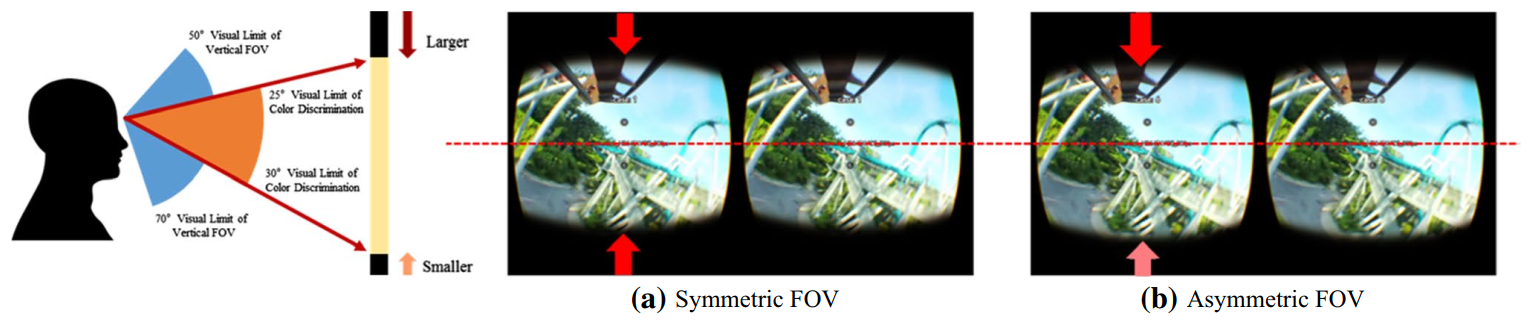
\includegraphics[width=\textwidth]{content/4_2_fovVignette/img/Asymmetrical_Vignette[Lim2020]}
    \caption{Asymmetrical FoV Limitation as proposed by Lim et al.~\cite{Lim2020}.}
    \label{fig:fov-assymetrical-vignette}
\end{figure}
Lim et al.~\cite{Lim2020} proposed in their study that the FoV vignetting should be applied asymmetrically, as human
visual characteristics produce an asymmetrical field of view with visual limits of 50\textdegree upwards and
70\textdegree downwards~\cite{Hatada1980}.
Since the horizontal field of view is significantly wider than the vertical field, we added an option to asymmetrically
limit the vertical field of view and forego any limitation of the horizontal visual field.
The fragment shader for the vertical vignette functions the same as their respective versions for the round
vignettes.
However, the calculation of the distance from the fragment to the center ignores the x-component as depicted below:
\begin{minted}{c}
    float dist = 0;
    if (vPosition.y > 0) { dist = vPosition.y; }
    else { dist = vPosition.y * -(0.7); }
\end{minted}
instead of calculating the euclidean distance, the distance above the center is the vertical position of the fragment
from the center.
The distance below the center is multiplied by $0.7$ to result in a smaller distance, and thus a smaller vignette on
the bottom, as depicted in figure~\ref{fig:fov-assymetrical-vignette}.
This feature is implemented experimentally, mainly because Lim et al.\ implemented an asymmetrical FoV Limitation in
their study, but no symmetrical limitation.
We understand that Lim et al.\ as well as their reference Hatada, Sakata, and Kusaka~\cite{Hatada1980} argue for an
asymmetrical FoV vignette as it is based on human visual characteristics, and is therefore less noticeable.
However, an asymmetrical vignette could lead to users not focusing on the center of the HMD's lenses but slightly
below, leading to unfocused images that may increase cybersickness symptoms.
